\documentclass{standalone}
\usepackage{tikz}
\usetikzlibrary{patterns, positioning}


\begin{document}
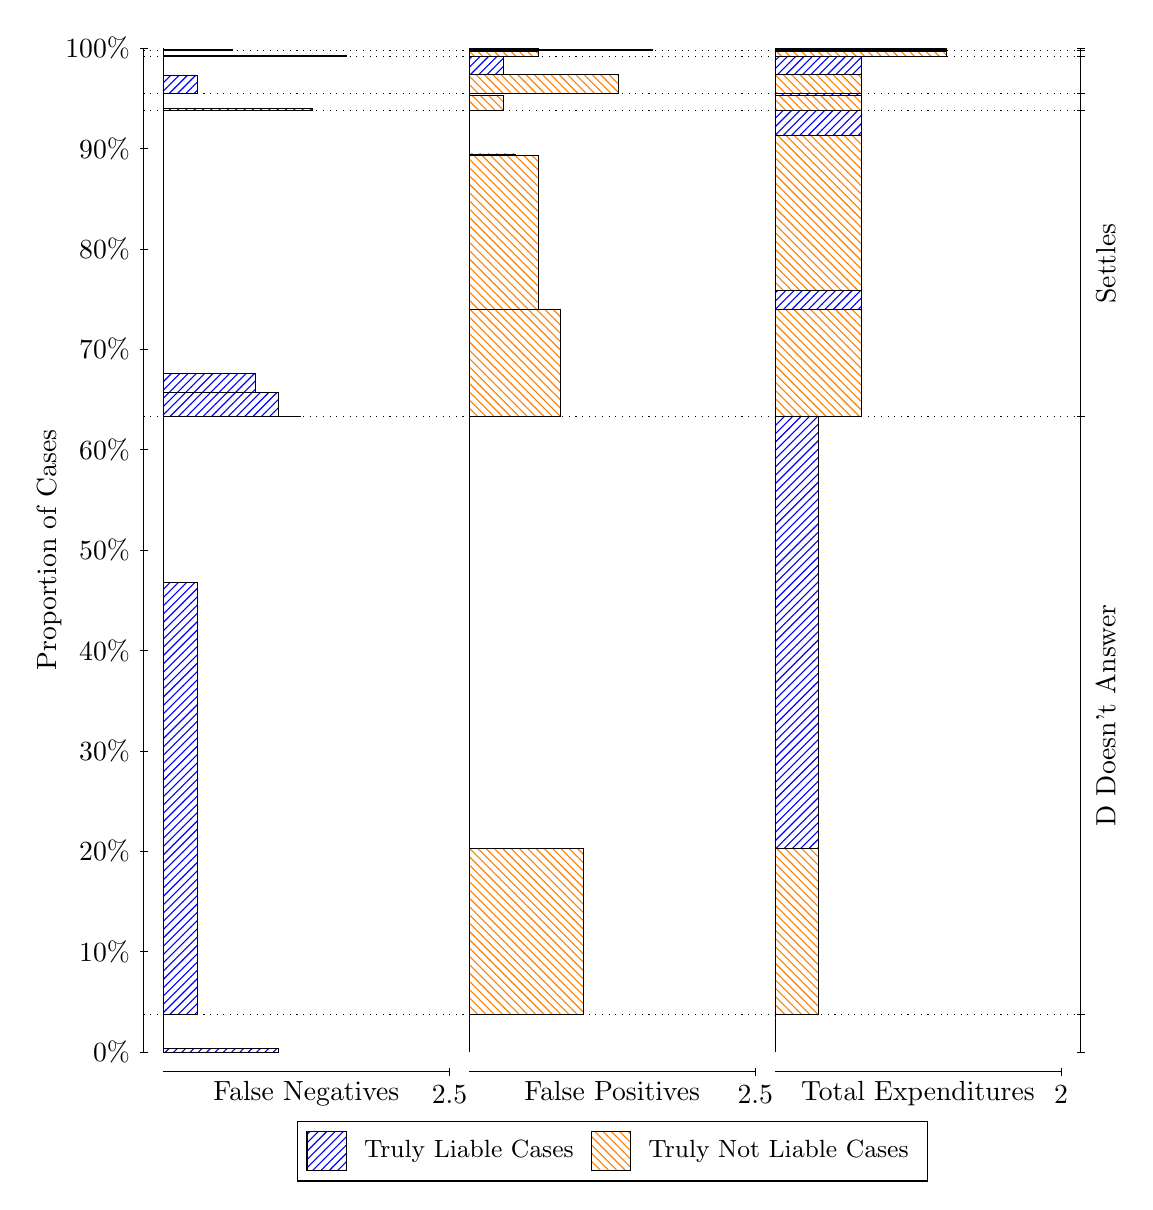
\begin{tikzpicture}
\draw[black, very thin] (1.5,1.75) -- (1.5,14.5);
\node[rotate=90, text=black, anchor=center] at (0.3, 8.125) {Proportion of Cases};
\draw[black, very thin] (1.45,1.75) -- (1.55,1.75);
\node[text=black, anchor=east] at (1.45, 1.75) {0\%};
\draw[black, very thin] (1.45,3.025) -- (1.55,3.025);
\node[text=black, anchor=east] at (1.45, 3.025) {10\%};
\draw[black, very thin] (1.45,4.3) -- (1.55,4.3);
\node[text=black, anchor=east] at (1.45, 4.3) {20\%};
\draw[black, very thin] (1.45,5.575) -- (1.55,5.575);
\node[text=black, anchor=east] at (1.45, 5.575) {30\%};
\draw[black, very thin] (1.45,6.85) -- (1.55,6.85);
\node[text=black, anchor=east] at (1.45, 6.85) {40\%};
\draw[black, very thin] (1.45,8.125) -- (1.55,8.125);
\node[text=black, anchor=east] at (1.45, 8.125) {50\%};
\draw[black, very thin] (1.45,9.4) -- (1.55,9.4);
\node[text=black, anchor=east] at (1.45, 9.4) {60\%};
\draw[black, very thin] (1.45,10.675) -- (1.55,10.675);
\node[text=black, anchor=east] at (1.45, 10.675) {70\%};
\draw[black, very thin] (1.45,11.95) -- (1.55,11.95);
\node[text=black, anchor=east] at (1.45, 11.95) {80\%};
\draw[black, very thin] (1.45,13.225) -- (1.55,13.225);
\node[text=black, anchor=east] at (1.45, 13.225) {90\%};
\draw[black, very thin] (1.45,14.5) -- (1.55,14.5);
\node[text=black, anchor=east] at (1.45, 14.5) {100\%};

\draw[black, very thin] (13.4,1.75) -- (13.4,14.5);
\draw[black, very thin] (13.35,1.75) -- (13.45,1.75);
\node[anchor=west] at (13.35, 1.75) {};
\draw[black, very thin] (13.35,2.2245) -- (13.45,2.2245);
\node[anchor=west] at (13.35, 2.2245) {};
\draw[black, very thin] (13.35,9.8205) -- (13.45,9.8205);
\node[anchor=west] at (13.35, 9.8205) {};
\draw[black, very thin] (13.35,13.705) -- (13.45,13.705);
\node[anchor=west] at (13.35, 13.705) {};
\draw[black, very thin] (13.35,13.921) -- (13.45,13.921);
\node[anchor=west] at (13.35, 13.921) {};
\draw[black, very thin] (13.35,14.395) -- (13.45,14.395);
\node[anchor=west] at (13.35, 14.395) {};
\draw[black, very thin] (13.35,14.469) -- (13.45,14.469);
\node[anchor=west] at (13.35, 14.469) {};
\draw[black, very thin] (13.35,14.5) -- (13.45,14.5);
\node[anchor=west] at (13.35, 14.5) {};

\draw[black, very thin, pattern color=blue, pattern=north east lines] (1.75,1.75) rectangle (3.2033,1.7999);
\draw[black, very thin, pattern color=orange, pattern=north west lines] (1.75,1.7999) rectangle (1.75,2.2245);
\draw[black, very thin, pattern color=blue, pattern=north east lines] (1.75,2.2245) rectangle (2.186,7.7108);
\draw[black, very thin, pattern color=orange, pattern=north west lines] (1.75,7.7108) rectangle (1.75,9.8205);
\draw[black, very thin, pattern color=blue, pattern=north east lines] (1.75,9.8205) rectangle (3.494,9.8229);
\draw[black, very thin, pattern color=blue, pattern=north east lines] (1.75,9.8229) rectangle (3.2033,10.128);
\draw[black, very thin, pattern color=blue, pattern=north east lines] (1.75,10.128) rectangle (2.9127,10.369);
\draw[black, very thin, pattern color=orange, pattern=north west lines] (1.75,10.369) rectangle (1.75,13.705);
\draw[black, very thin, pattern color=blue, pattern=north east lines] (1.75,13.705) rectangle (3.6393,13.732);
\draw[black, very thin, pattern color=orange, pattern=north west lines] (1.75,13.732) rectangle (1.75,13.921);
\draw[black, very thin, pattern color=blue, pattern=north east lines] (1.75,13.921) rectangle (2.186,14.154);
\draw[black, very thin, pattern color=orange, pattern=north west lines] (1.75,14.154) rectangle (1.75,14.395);
\draw[black, very thin, pattern color=blue, pattern=north east lines] (1.75,14.395) rectangle (4.0753,14.411);
\draw[black, very thin, pattern color=orange, pattern=north west lines] (1.75,14.411) rectangle (1.75,14.469);
\draw[black, very thin, pattern color=blue, pattern=north east lines] (1.75,14.469) rectangle (2.622,14.484);
\draw[black, very thin, pattern color=orange, pattern=north west lines] (1.75,14.484) rectangle (1.75,14.5);
\draw[black, very thin, pattern color=orange, pattern=north west lines] (5.6333,1.75) rectangle (5.6333,2.1746);
\draw[black, very thin, pattern color=blue, pattern=north east lines] (5.6333,2.1746) rectangle (5.6333,2.2245);
\draw[black, very thin, pattern color=orange, pattern=north west lines] (5.6333,2.2245) rectangle (7.0867,4.3341);
\draw[black, very thin, pattern color=blue, pattern=north east lines] (5.6333,4.3341) rectangle (5.6333,9.8205);
\draw[black, very thin, pattern color=orange, pattern=north west lines] (5.6333,9.8205) rectangle (6.796,11.179);
\draw[black, very thin, pattern color=orange, pattern=north west lines] (5.6333,11.179) rectangle (6.5053,13.135);
\draw[black, very thin, pattern color=orange, pattern=north west lines] (5.6333,13.135) rectangle (6.2147,13.157);
\draw[black, very thin, pattern color=blue, pattern=north east lines] (5.6333,13.157) rectangle (5.6333,13.705);
\draw[black, very thin, pattern color=orange, pattern=north west lines] (5.6333,13.705) rectangle (6.0693,13.895);
\draw[black, very thin, pattern color=blue, pattern=north east lines] (5.6333,13.895) rectangle (5.6333,13.921);
\draw[black, very thin, pattern color=orange, pattern=north west lines] (5.6333,13.921) rectangle (7.5227,14.163);
\draw[black, very thin, pattern color=blue, pattern=north east lines] (5.6333,14.163) rectangle (6.0693,14.395);
\draw[black, very thin, pattern color=orange, pattern=north west lines] (5.6333,14.395) rectangle (6.5053,14.453);
\draw[black, very thin, pattern color=blue, pattern=north east lines] (5.6333,14.453) rectangle (5.6333,14.469);
\draw[black, very thin, pattern color=orange, pattern=north west lines] (5.6333,14.469) rectangle (7.9587,14.485);
\draw[black, very thin, pattern color=blue, pattern=north east lines] (5.6333,14.485) rectangle (6.5053,14.5);
\draw[black, very thin, pattern color=orange, pattern=north west lines] (9.5167,1.75) rectangle (9.5167,2.1746);
\draw[black, very thin, pattern color=blue, pattern=north east lines] (9.5167,2.1746) rectangle (9.5167,2.2245);
\draw[black, very thin, pattern color=orange, pattern=north west lines] (9.5167,2.2245) rectangle (10.062,4.3341);
\draw[black, very thin, pattern color=blue, pattern=north east lines] (9.5167,4.3341) rectangle (10.062,9.8205);
\draw[black, very thin, pattern color=orange, pattern=north west lines] (9.5167,9.8205) rectangle (10.607,11.179);
\draw[black, very thin, pattern color=blue, pattern=north east lines] (9.5167,11.179) rectangle (10.607,11.419);
\draw[black, very thin, pattern color=orange, pattern=north west lines] (9.5167,11.419) rectangle (10.607,13.397);
\draw[black, very thin, pattern color=blue, pattern=north east lines] (9.5167,13.397) rectangle (10.607,13.705);
\draw[black, very thin, pattern color=orange, pattern=north west lines] (9.5167,13.705) rectangle (10.607,13.895);
\draw[black, very thin, pattern color=blue, pattern=north east lines] (9.5167,13.895) rectangle (10.607,13.921);
\draw[black, very thin, pattern color=orange, pattern=north west lines] (9.5167,13.921) rectangle (10.607,14.163);
\draw[black, very thin, pattern color=blue, pattern=north east lines] (9.5167,14.163) rectangle (10.607,14.395);
\draw[black, very thin, pattern color=orange, pattern=north west lines] (9.5167,14.395) rectangle (11.697,14.453);
\draw[black, very thin, pattern color=blue, pattern=north east lines] (9.5167,14.453) rectangle (11.697,14.469);
\draw[black, very thin, pattern color=orange, pattern=north west lines] (9.5167,14.469) rectangle (11.697,14.485);
\draw[black, very thin, pattern color=blue, pattern=north east lines] (9.5167,14.485) rectangle (11.697,14.5);
\draw[black, dotted] (1.5,2.2245) -- (13.4,2.2245);
\draw[black, dotted] (1.5,9.8205) -- (13.4,9.8205);
\draw[black, dotted] (1.5,13.705) -- (13.4,13.705);
\draw[black, dotted] (1.5,13.921) -- (13.4,13.921);
\draw[black, dotted] (1.5,14.395) -- (13.4,14.395);
\draw[black, dotted] (1.5,14.469) -- (13.4,14.469);
\draw[black, very thin] (1.75,1.5) -- (5.3833,1.5);
\node[text=black, anchor=north] at (3.5667, 1.5) {False Negatives};
\draw[black, very thin] (5.3833,1.45) -- (5.3833,1.55);
\node[text=black, anchor=north] at (5.3833, 1.45) {2.5};

\draw[black, very thin] (5.6333,1.5) -- (9.2667,1.5);
\node[text=black, anchor=north] at (7.45, 1.5) {False Positives};
\draw[black, very thin] (9.2667,1.45) -- (9.2667,1.55);
\node[text=black, anchor=north] at (9.2667, 1.45) {2.5};

\draw[black, very thin] (9.5167,1.5) -- (13.15,1.5);
\node[text=black, anchor=north] at (11.333, 1.5) {Total Expenditures};
\draw[black, very thin] (13.15,1.45) -- (13.15,1.55);
\node[text=black, anchor=north] at (13.15, 1.45) {2};


\node[text=black, centered, rotate=90] at (13.72, 6.0225) {D Doesn't Answer};
\node[text=black, centered, rotate=90] at (13.72, 11.763) {Settles};





\draw (7.449999999999999,1.5) node[draw=none] (baseCoordinate) {};
\begin{scope}[align=center]
        \matrix[scale=0.5, draw=black, below=0.5cm of baseCoordinate, nodes={draw}, column sep=0.1cm]{
            \node[rectangle, draw, minimum width=0.5cm, minimum height=0.5cm, pattern color=blue, pattern=north east lines] {}; &
            \node[draw=none, font=\small, text=black] (B) {Truly Liable Cases}; &
            \node[rectangle, draw, minimum width=0.5cm, minimum height=0.5cm, pattern color=orange, pattern=north west lines] {}; &
            \node[draw=none, font=\small, text=black] (B) {Truly Not Liable Cases}; \\
            };
\end{scope}

\end{tikzpicture}
\end{document}